\documentclass[aps, superscriptaddress, notitlepage]{revtex4-1}
\usepackage{amsmath,amsfonts,amssymb,graphicx,hyperref,listings,xcolor,float}
\usepackage[ddmmyyyy, 24hr]{datetime}

% tikz
\usepackage{tikz}
\usetikzlibrary{calc}
\usetikzlibrary{arrows.meta,arrows}

% (pseudo-)algorithms [seems to need `lualatex` when this is actually used in the document]
% https://tex.stackexchange.com/questions/70181
\usepackage{algcompatible,newfloat,etoolbox}
\AtEndEnvironment{algorithm}{\noindent\hrulefill\par\nobreak\vskip-5pt}
\DeclareFloatingEnvironment[fileext=loa, listname=List of Algorithms, name=ALG., placement=tbhp]{algorithm}
% https://tex.stackexchange.com/questions/353132
\algrenewcommand\algorithmicrequire{\textbf{Input:}}
\algrenewcommand\algorithmicensure{\textbf{Output:}}
% https://tex.stackexchange.com/questions/180212
\algrenewcommand{\algorithmiccomment}[2][.6\linewidth]{\leavevmode\hfill\makebox[#1][l]{\triangleright~{\em#2}}}
% https://tex.stackexchange.com/questions/184827
\providecommand{\LINECOMMENT}[1]{\STATEx//~{\em#1}}

% colours
% seaborn `colorblind' palette
% https://seaborn.pydata.org/tutorial/color_palettes.html
\definecolor{purple}{HTML}{CC78BC}
\definecolor{green}{HTML}{029E73}
\definecolor{blue}{HTML}{0173B2}
\definecolor{lightblue}{HTML}{56B4E9}
\definecolor{yellow}{HTML}{DE8F05}
\definecolor{brown}{HTML}{CA9161}
\definecolor{red}{HTML}{D55E00}
\definecolor{grey}{HTML}{949494}
\definecolor{pink}{HTML}{FBAFE4}
\definecolor{lightyellow}{HTML}{ECE133}

% header/footer
% https://tex.stackexchange.com/questions/117402
\usepackage{fancyhdr} 
\cfoot{\thepage}
\pagestyle{fancy}
% https://tex.stackexchange.com/questions/40172
\renewcommand{\headrulewidth}{0pt}
\fancyhead{}

%%%%% MACROS

\def\scale{0.8}
\providecommand\RETURN{\STATE\textbf{return}~}
\providecommand\ASSERT{\STATE\textbf{assert}~}
\providecommand\BREAK{\STATE\textbf{break}~}
\providecommand\TRUE{\textsc{true}}
\providecommand\FALSE{\textsc{false}}



%%%%% DOCUMENT

\begin{document}

%%%%% TITLE

\title{Forces in vertex models}
\author{Yann-Edwin Keta}
\date{\today, \currenttime}
\maketitle

%%%%% CONTENT

\section{Cell potential energy}

We introduce for each cell $i$ a reference perimeter $P^0_i$ and a reference area $A^0_i$, and for each of its cell corner $\mu \in \Omega_i$ a force whose effect is to bring the cell's perimeter $P_i$ and area $A_i$ to their reference quantities. A possible force derives from the following potential energy \cite{farhadifar2007influence,fletcher2014vertex,bi2016motilitydriven,sknepnek2023generating}
\begin{equation}
E_{\mathrm{VM}} = \sum_{\text{cells } i} \left[\frac{1}{2} K_i (A_i - A_i^0)^2 + \frac{1}{2} \Gamma_i (P_i - P_i^0)^2\right],
\label{eq:evm}
\end{equation}
where $K_i$ and $\Gamma_i$ are respectively area and perimeter elastic constants. We denote $\boldsymbol{r}_{\mu}$, $\boldsymbol{r}_i$ the position of vertices $\mu, i$ (see Fig.~\ref{fig:fmu}). The cell's perimeter can be written
\begin{equation}
P_i = \sum_{\mu \in \Omega_i} |\boldsymbol{r}_{\mu} - \boldsymbol{r}_{\mu - 1}|,
\end{equation}
and the cell's area can be computed with the shoelace formula
\begin{equation}
A_i = \sum_{\mu \in \Omega_i} \frac{1}{2} [(\boldsymbol{r}_{\mu} - \boldsymbol{r}_{i}) \times (\boldsymbol{r}_{\mu - 1} - \boldsymbol{r}_{i})] \cdot \hat{\boldsymbol{e}}_z.
\end{equation}
Note that, by convention of ordering of cell corners, each term in this sum \textit{must be} positive. With these notations, we thus write the force acting on vertex $\mu$
\begin{equation}
\boldsymbol{F}_{\mathrm{VM},\mu} = -\nabla_{\mu} E_{\mathrm{VM}},
\label{eq:fmugrade}
\end{equation}
where $\nabla_{\mu} \equiv \partial/\partial \boldsymbol{r}_{\mu}$. We compute
\begin{equation}
\nabla_{\mu} \left(|\boldsymbol{r}_{\mu} - \boldsymbol{r}_{\mu - 1}|\right) = \frac{\boldsymbol{r}_{\mu} - \boldsymbol{r}_{\mu - 1}}{|\boldsymbol{r}_{\mu} - \boldsymbol{r}_{\mu - 1}|},
\end{equation}
as well as
\begin{equation}
\nabla_{\mu} \left([(\boldsymbol{r}_{\mu} - \boldsymbol{r}_i) \times (\boldsymbol{r}_{\mu - 1} - \boldsymbol{r}_i)] \cdot \hat{\boldsymbol{e}}_z\right) = (\boldsymbol{r}_{\mu - 1} - \boldsymbol{r}_i) \times \hat{\boldsymbol{e}}_z
\end{equation}
to write \eqref{eq:fmugrade} in its full form
\begin{equation}
\begin{aligned}
\boldsymbol{F}_{\mathrm{VM},\mu} &= - \sum_{\text{cells i},~ \mu \in \Omega_i} \bigg[\frac{1}{2} K_i (A_i - A^0_i) \left[(\boldsymbol{r}_{\mu + 1} - \boldsymbol{r}_i) \times \hat{\boldsymbol{e}}_z - (\boldsymbol{r}_{\mu - 1} - \boldsymbol{r}_i) \times \hat{\boldsymbol{e}}_z\right]\\
&\qquad\qquad\qquad\qquad+ \Gamma_i (P_i - P^0_i) \left[\frac{\boldsymbol{r}_{\mu} - \boldsymbol{r}_{\mu - 1}}{|\boldsymbol{r}_{\mu} - \boldsymbol{r}_{\mu - 1}|} + \frac{\boldsymbol{r}_{\mu} - \boldsymbol{r}_{\mu - 1}}{|\boldsymbol{r}_{\mu} - \boldsymbol{r}_{\mu - 1}|}\right]\bigg]\\
&= \sum_{\text{cells i},~ \mu \in \Omega_i} \bigg[\frac{1}{2} K_i (A_i - A^0_i) {\color{blue} \underbrace{(\boldsymbol{r}_{\mu - 1} - \boldsymbol{r}_{\mu + 1}) \times \hat{\boldsymbol{e}}_z}_{\text{towards cell interior}}} + \Gamma_i (P_i - P^0_i) \bigg[{\color{purple} \underbrace{\frac{\boldsymbol{r}_{\mu - 1} - \boldsymbol{r}_{\mu}}{|\boldsymbol{r}_{\mu - 1} - \boldsymbol{r}_{\mu}|}}_{\text{towards neighbour}}} + {\color{purple} \underbrace{\frac{\boldsymbol{r}_{\mu + 1} - \boldsymbol{r}_{\mu}}{|\boldsymbol{r}_{\mu + 1} - \boldsymbol{r}_{\mu}|}}_{\text{towards neighbour}}}\bigg]\bigg],
\end{aligned}
\end{equation}
where underbraced vectors are represented in Fig.~\ref{fig:fmu}. It is noteworthy that, with potential \eqref{eq:evm}, the force acting on each cell centre is zero
\begin{equation}
\boldsymbol{F}_{\mathrm{VM}, i} = - \nabla_i E_{\mathrm{VM}} = - \frac{1}{2} K_i (A_i - A^0_i) \sum_{\mu \in \Omega_i} (\boldsymbol{r}_{\mu} - \boldsymbol{r}_{\mu - 1}) \times \hat{\boldsymbol{e}}_z = 0.
\end{equation}

\begin{figure}[!t]
\centering
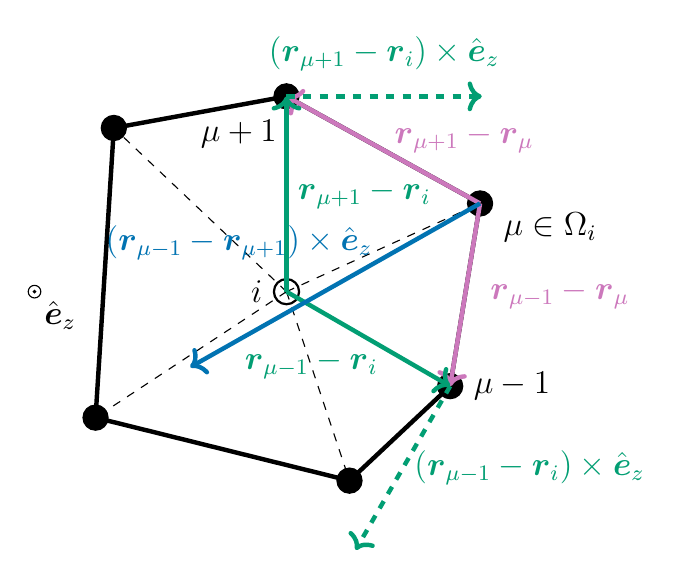
\begin{tikzpicture}[scale=\scale]
% FIRST CELL
% cell centre
\coordinate (A) at (0, 0);
\draw[thick] (A) circle (0.2) node[left,xshift=-5pt]{\large $i$};
% cell corners
\coordinate (B) at ($(A) + ({4*cos(30 + 0.2*60) + 0.1}, {3*sin(30 + 0*60) - 0.1})$);
\draw[fill=black] (B) circle (0.2) node[below right,xshift=5pt]{\large $\mu \in \Omega_i$};
\coordinate (C) at ($(A) + ({2.9*cos(30 + 1*60)}, {3.1*sin(30 + 1*60)})$);
\draw[fill=black] (C) circle (0.2) node[below left,yshift=-5pt]{\large $\mu + 1$};
\coordinate (D) at ($(A) + ({3*cos(30 + 2.1*60)}, {3*sin(30 + 1.5*60)})$);
\draw[fill=black] (D) circle (0.2);
\coordinate (E) at ($(A) + ({3.5*cos(30 + 3*60)}, {4*sin(30 + 3*60)})$);
\draw[fill=black] (E) circle (0.2);
\coordinate (F) at ($(A) + ({1 + 3*cos(30 + 4*60)}, {3*sin(30 + 4*60)})$);
\draw[fill=black] (F) circle (0.2);
\coordinate (G) at ($(A) + ({3*cos(30 + 5*60)}, {3*sin(30 + 5*60)})$);
\draw[fill=black] (G) circle (0.2) node[right,xshift=5pt]{\large $\mu - 1$};
% junctions
\draw[ultra thick] (B) -- (C) -- (D) -- (E) -- (F) -- (G) -- (B);
% inner edges
\draw[dashed] (A) -- (B);
\draw[dashed] (A) -- (C);
\draw[dashed] (A) -- (D);
\draw[dashed] (A) -- (E);
\draw[dashed] (A) -- (F);
\draw[dashed] (A) -- (G);

\draw (-4, 0) circle (0.1) node[below right]{\large $\hat{\boldsymbol{e}}_z$};
\draw[fill=black] (-4, 0) circle (0.02);

% perimeter term
\draw[purple, ultra thick, ->] (B) -- (C) node[midway, above right, xshift=0pt, yshift=-5pt]{\large $\boldsymbol{r}_{\mu + 1} - \boldsymbol{r}_{\mu}$};
\draw[purple, ultra thick, ->] (B) -- (G) node[midway, right, xshift=5pt]{\large $\boldsymbol{r}_{\mu - 1} - \boldsymbol{r}_{\mu}$};

% area term
\draw[green, ultra thick, ->] (A) -- (C) node[midway, right]{\large $\boldsymbol{r}_{\mu + 1} - \boldsymbol{r}_i$};
\draw[green, ultra thick, ->] (A) -- (G) node[midway, below left, xshift=7.5pt]{\large $\boldsymbol{r}_{\mu - 1} - \boldsymbol{r}_i$};
% https://tex.stackexchange.com/a/63569
\draw[green, ultra thick, dashed, ->] let \p{A}=(A), \p{C}=(C) in (C) -- ++({\y{C} - \y{A}}, {-(\x{C} - \x{A})}) node[midway, above, yshift=5pt]{\large $(\boldsymbol{r}_{\mu + 1} - \boldsymbol{r}_i) \times \hat{\boldsymbol{e}}_z$};
\draw[green, ultra thick, dashed, ->] let \p{A}=(A), \p{G}=(G) in (G) -- ++({\y{G} - \y{A}}, {-(\x{G} - \x{A})}) node[midway, right, yshift=0pt]{\large $(\boldsymbol{r}_{\mu - 1} - \boldsymbol{r}_i) \times \hat{\boldsymbol{e}}_z$};
\draw[blue, ultra thick, ->] let \p{C}=(C), \p{G}=(G) in (B) -- ++({-(\y{C} - \y{G})}, {(\x{C} - \x{G})}) node[midway, above left, xshift=17.5pt, yshift=5pt]{\large $(\boldsymbol{r}_{\mu - 1} - \boldsymbol{r}_{\mu + 1}) \times \hat{\boldsymbol{e}}_z$};

\end{tikzpicture}
\caption{Vertex representation of a single cell. By convention, cell centres are denoted by latin indices, and cell corners are denotes by greek indices. We denote $\Omega_i$ the ensemble of cell corners $\mu$ of the cell whose centre is $i$. By convention, $\mu + 1$ (respectively $\mu - 1$) denotes the next cell corner of $i$ after $\mu$ in anticlockwise (respectively clockwise) order.}
\label{fig:fmu}
\end{figure}

\bibliography{ref}

\end{document}

